\section{實驗與實體驗證}

\subsection{機器人定位與避障任務}

本研究先以微小化平台測試所建置的感測塔、系統與演算法,將於期末報告對大型無人載具(地面與水面)平台進行測試。

\paragraph{定位準確度測試}

本計畫先針對機器人定位的準確度逕行測試,測試方法比較 1) GPS與IMU進行感測融合,2) 只有GPU資料,實驗地點為交大圖書館前方空地,以一個邊長約100公尺的矩形路線,實驗人員攜帶所建置的感測塔跟著矩形路線行走,並將資料錄製於ROS Bag檔案,實驗結果如圖
\ref{table:loop_closure_error}所示。結果顯示,從出發點經過指定路線後,回到原始點的誤差值在兩組硬體設定相差不大,但於GPU+IMU設定標準差的值較小,表示在定位過程較穩定。

\begin{table}[h]
	\centering
	\begin{tabular}{| c| c| c|}
		\hline
		Sensor Set & 定位誤差  x, y (m) & 路線標準差 x, y (m) \\ \hline
		GPS + IMU & 0.65, 0.83 & 0.37, 0.42 \\ \hline
		GPS only  & 0.60, 0.83 & 0.41, 0.72 \\ \hline 
	\end{tabular}
	\caption{定位測試}
	\label{table:loop_closure_error}
\end{table} 

\paragraph{避障測試於簡化實驗環境} 

本計畫先使用微小化平台,先於室內與室外較為平坦之場域測試,測試內容(請參考圖~ \ref{figure:exp-results})與影片連結如下:

\begin{itemize}

\item
巡邏點進行純追蹤演算法(Pure Pursuit Algorithm): 
\url{https://youtu.be/DdaZkm7_bjI}

\item
避障實驗一(靜態障礙物): 
\url{https://youtu.be/ve4Mln4D1xo}

\item
避障實驗二(動態障礙物):
\url{https://youtu.be/E1anLPuXjxs}

\item
無人水上載具於虛擬環境避障任務: 
\url{https://youtu.be/DBuMrUvr7iY}

\end{itemize}

\begin{figure}[h] % h means put this image here
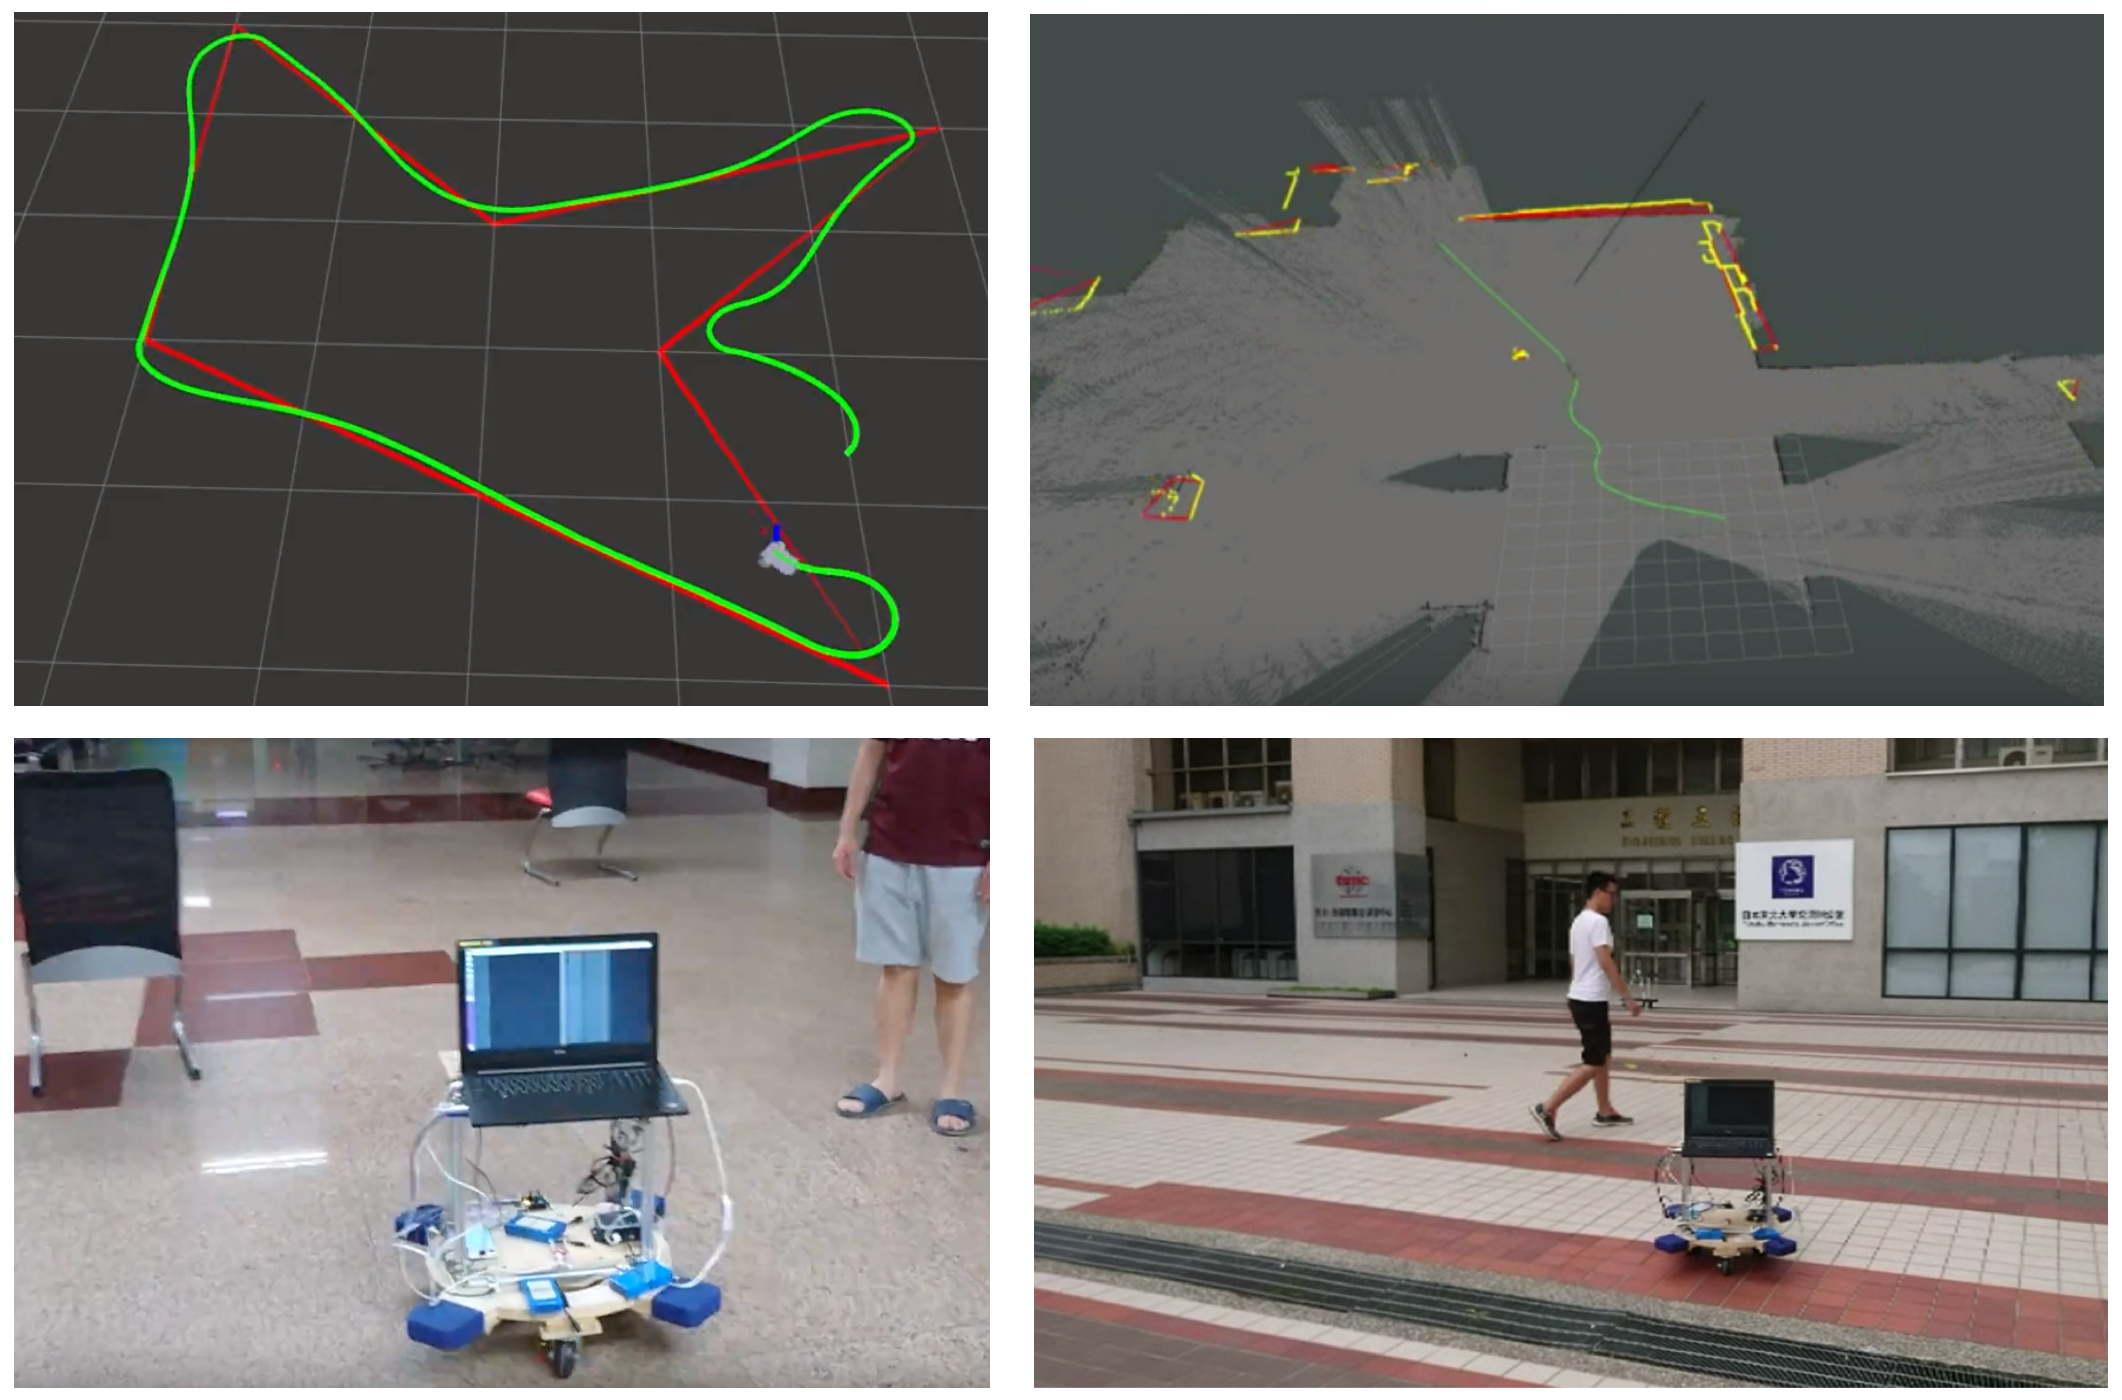
\includegraphics[width=\columnwidth]{images/exp-results.png}
\centering
\caption{微小化平台與簡化場域測試}
 \label{figure:exp-results}
\end{figure}


\subsection{地面無人載具(進行中)}

本計畫預計將所開發之演算法用於大型地面無人載具(Clearpath Husky,請參考圖~\ref{figure:ground-vehicle}),結合所開發的點雲及開發演算法於地形模擬建構,於不平坦之崎嶇地形進行測試。

\begin{figure}[h] % h means put this image here
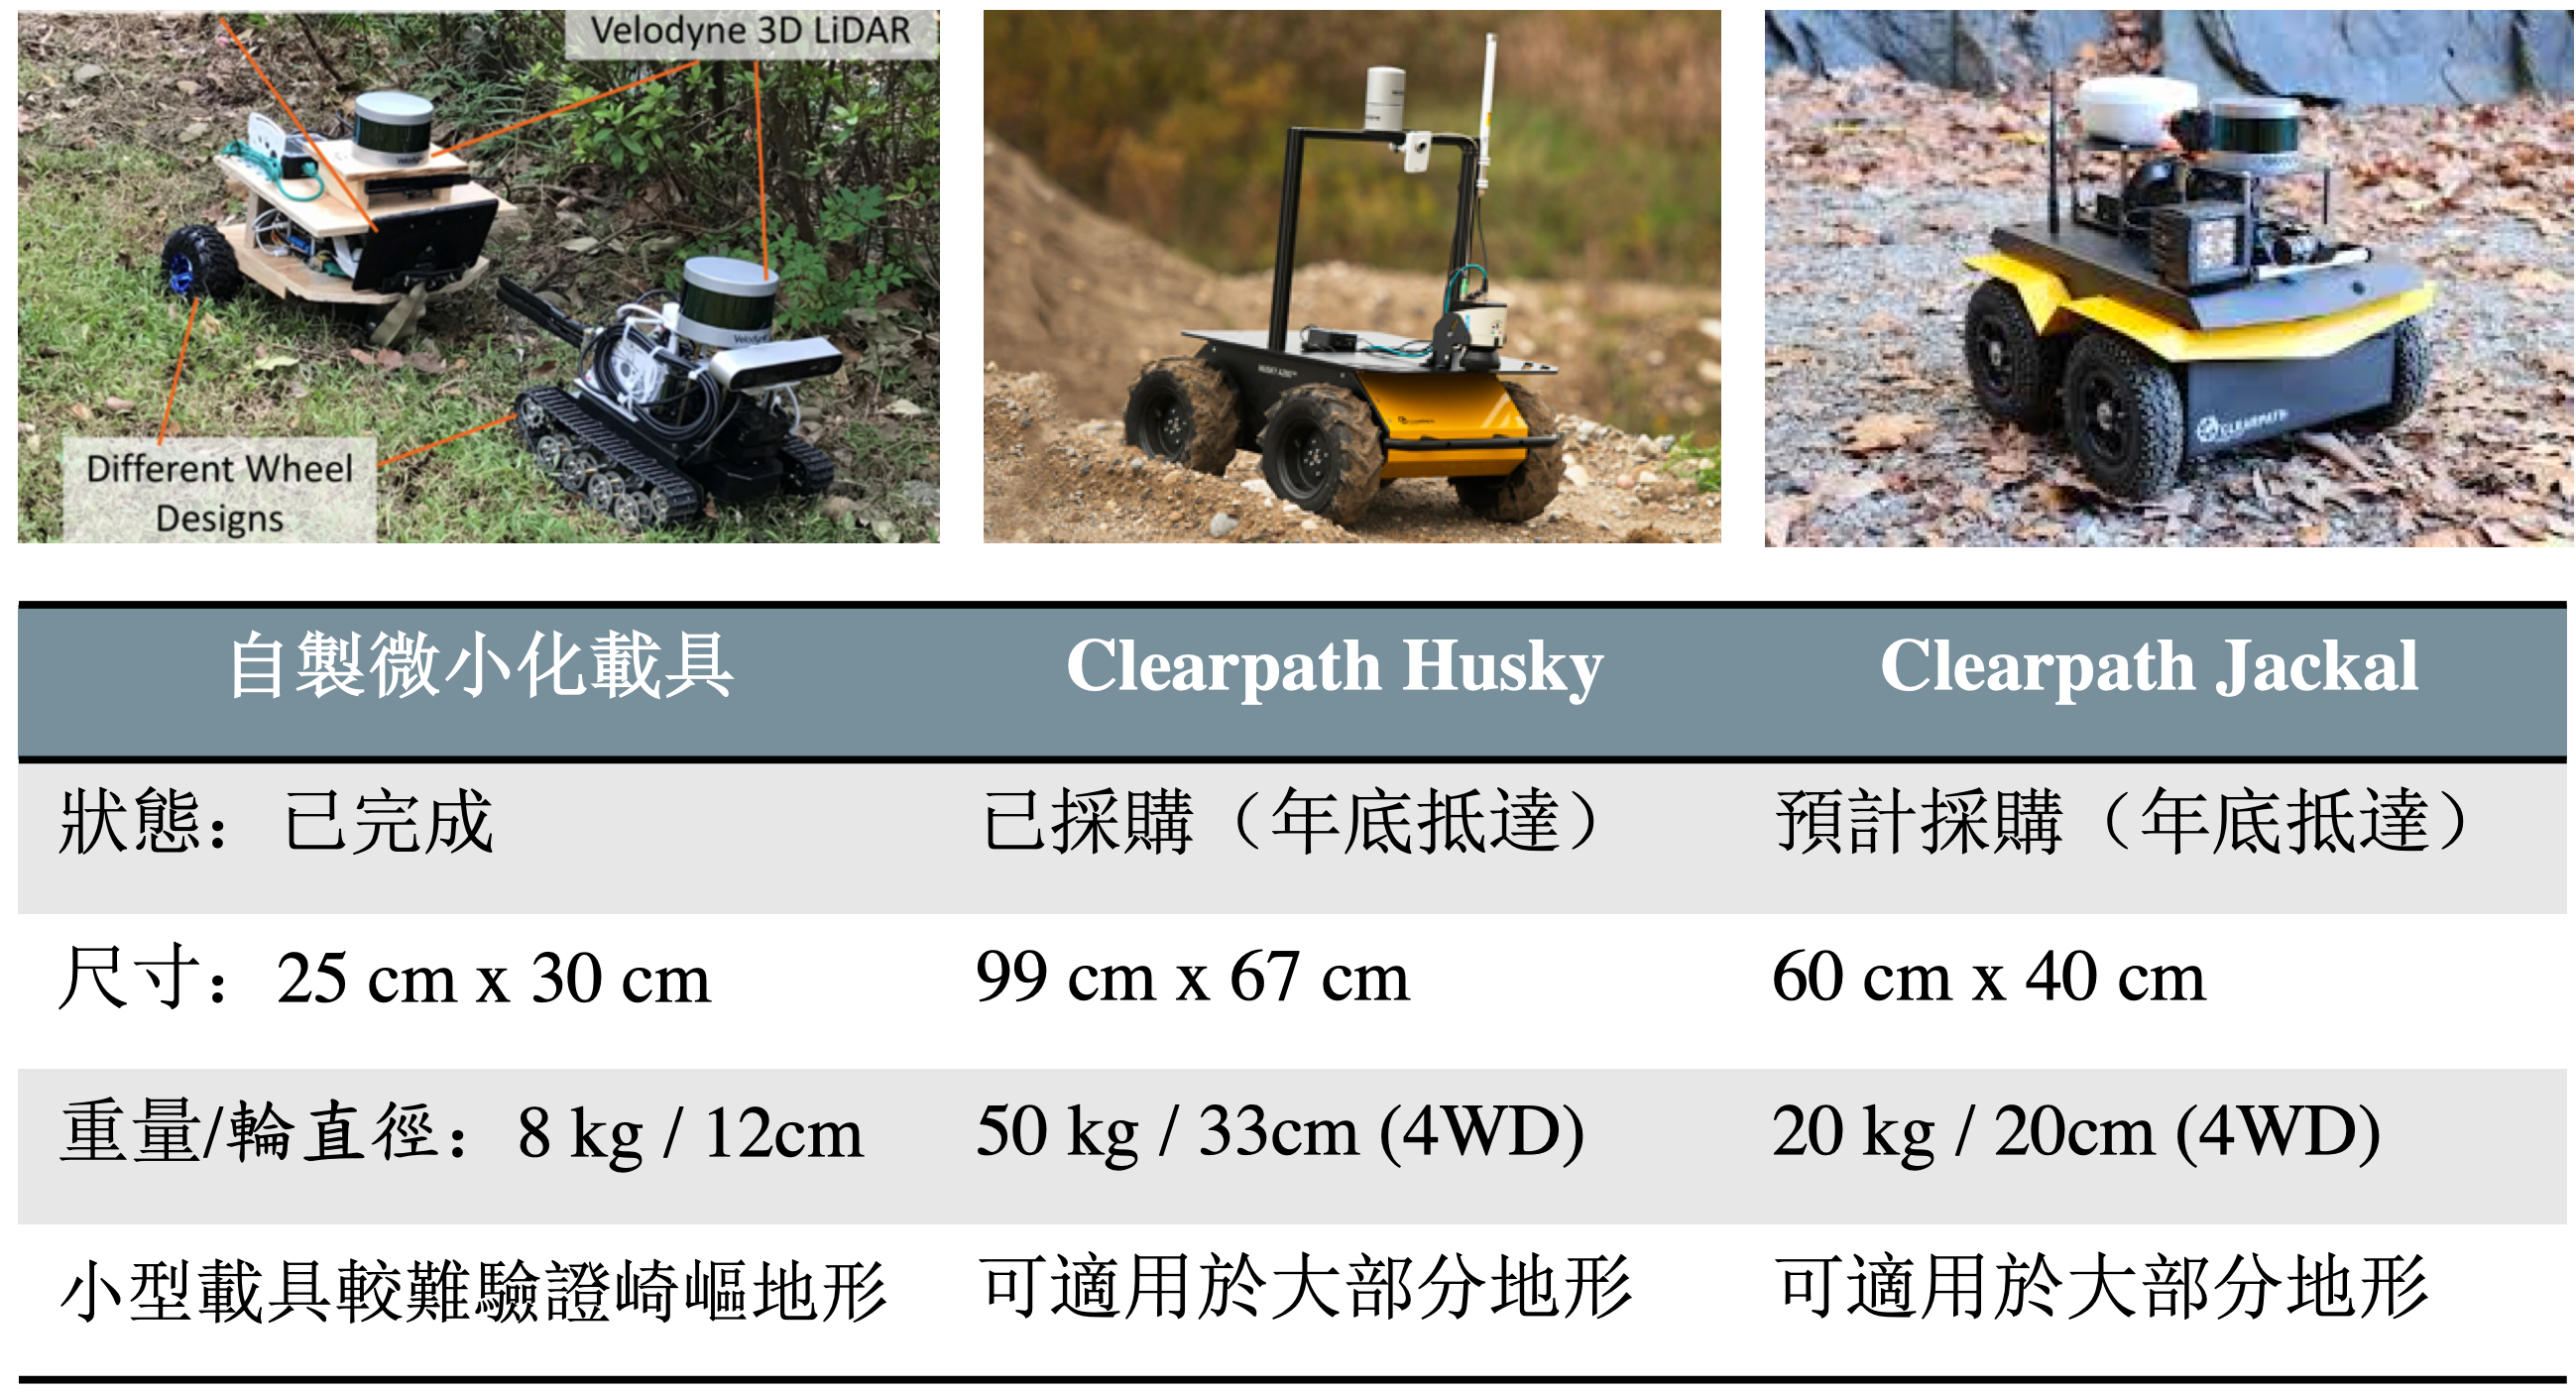
\includegraphics[width=\columnwidth]{images/ground-vehicle.png}
\centering
\caption{地面無人載具實際場域驗證}
 \label{figure:ground-vehicle}
\end{figure}

\subsection{水面無人載具與RobotX競賽(進行中)}

本計畫已將所開發之演算法用於大型水面無人載具,Marine Advanced Research 所提供的自適應性波浪快艇 (Wave Adaptive Modular Vessel, WAM-V),並透過設計此船隻的感測、計算、及動力完成競賽任務。本論文使用之自適應性波浪快艇系統架構圖如圖~\ref{figure:system_diagram}所示,其中主要分成三個部分: 硬體、電路、軟體,分別在模擬與實際竹湖場域測試。

\begin{figure}[bht]
	\centering
	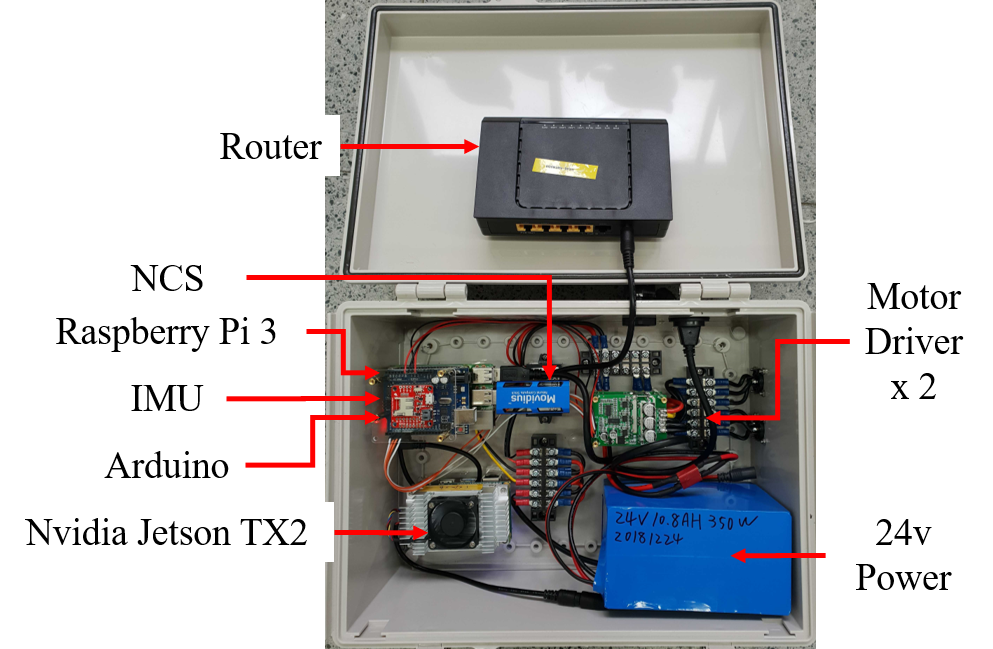
\includegraphics[height=!,width=\linewidth,keepaspectratio=true]
	{images/hardware_setting.png}
	\caption{本計畫將所開發的演算法移植到大型水上無人載具,將於2018年12月代表台灣第一次參與在夏威夷舉行的RobotX競賽。}
	\label{figure:system_diagram}
\end{figure}


